\chapter{相关理论基础}
[xxx]

\section{表格}

表应具有自明性。为使表格简洁易读,尽可能采用三线表,如表~\ref{tab:three-line}。

\begin{table}[H]
  \centering
  \caption{三线表示例}
  \begin{tabular}{ll}
    \toprule
    文件名          & 描述                         \\
    \midrule
    main.tex  & 入口文件 \\
    hnuthesis.cls   & 样式设置                     \\
    hnunumerical.bst & BibTeX 参考文献表样式文件    \\
    \bottomrule
  \end{tabular}
  \label{tab:three-line}
\end{table}

研究生要求使用英文小写字母 a、b、c……顺序编号。

\subsection{复杂一点}
latex 表格设置相对word 麻烦一些,比如表 ~\ref{table:test}。

\vspace{-10pt}
\begin{table}[H]  
\centering
\small
\caption{复杂一点点的表}
\label{table:test}  
\begin{tabular}{cccccccccc}  % 调整列数,以匹配内容  
\toprule  
\multicolumn{2}{c}{\multirow{3}{*}{\makecell[c]{目标}}} & \multicolumn{7}{c}{xxxx情况} & \multirow{3}{*}{$\beta$} \\  
\cline{3-9} % 在第3列到第6列之间划线  
 & & \makecell{项\\(1)} & \makecell{项\\(2)} & \makecell{项\\(3)} & \makecell{项\\(4)} & \makecell{项\\(5)} & \makecell{项\\(6)} & 项 & \\  
\midrule  
\multirow{3}{*}{\makecell[c]{任务1\\(xxx)}} & 子任务1 & 1 & 2 & 3 & 4 & 5 & 6 & 7 & 100\% \\  
 & 子任务2 & 1 & 2 & 3 & 4 & 5 & 6 & 7 & 100\% \\  
 & 子任务3 & 1 & 2 & 3 & 4 & 5 & 6 & 7 & 100\% \\  
 \multirow{3}{*}{\makecell[c]{任务1\\(xxx)}} & 子任务1 & 1 & 2 & 3 & 4 & 5 & 6 & 7 & 100\% \\  
 & 子任务2 & 1 & 2 & 3 & 4 & 5 & 6 & 7 & 100\% \\  
 & 子任务3 & 1 & 2 & 3 & 4 & 5 & 6 & 7 & 100\% \\  
\bottomrule  
\end{tabular}    
\end{table}  
\vspace{-10pt}

\section{图}

可以使用 pdf 格式的图,processon 能导出pdf,matplotlib 也能导出 pdf, 然后通过 pdfcandydt 进行裁剪。如图\ref{fig:img1}所示。

\vspace{-12pt}
\begin{figure}[H]
    \centering
    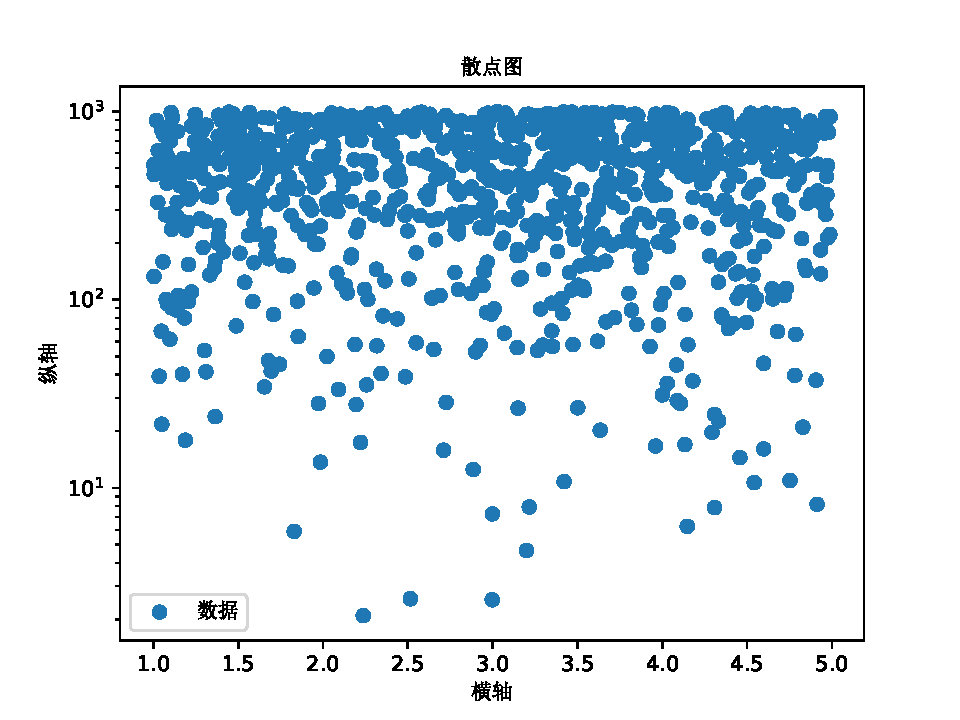
\includegraphics[width=0.6\linewidth]{figures/data/testA.pdf}
    \caption{图名}
    \label{fig:img1}
\end{figure}
\vspace{-18pt}

\subsection{子图}
如果一个图由两个或两个以上分图组成时,各分图分别以 (a)、(b)、(c)...... 作为图序,并须有分图题。
\begin{figure}[H] %这里使用的是强制位置,除非真的放不下,不然就是写在哪里图就放在哪里,不会乱动
	\centering  %图片全局居中
	\vspace{-0.35cm} %设置与上面正文的距离
	\subfigtopskip=2pt %设置子图与上面正文或别的内容的距离
	\subfigbottomskip=2pt %设置第二行子图与第一行子图的距离,即下面的头与上面的脚的距离
	\subfigcapskip=-5pt %设置子图与子标题之间的距离
	\subfigure[original]{
		\label{level.sub.1}
		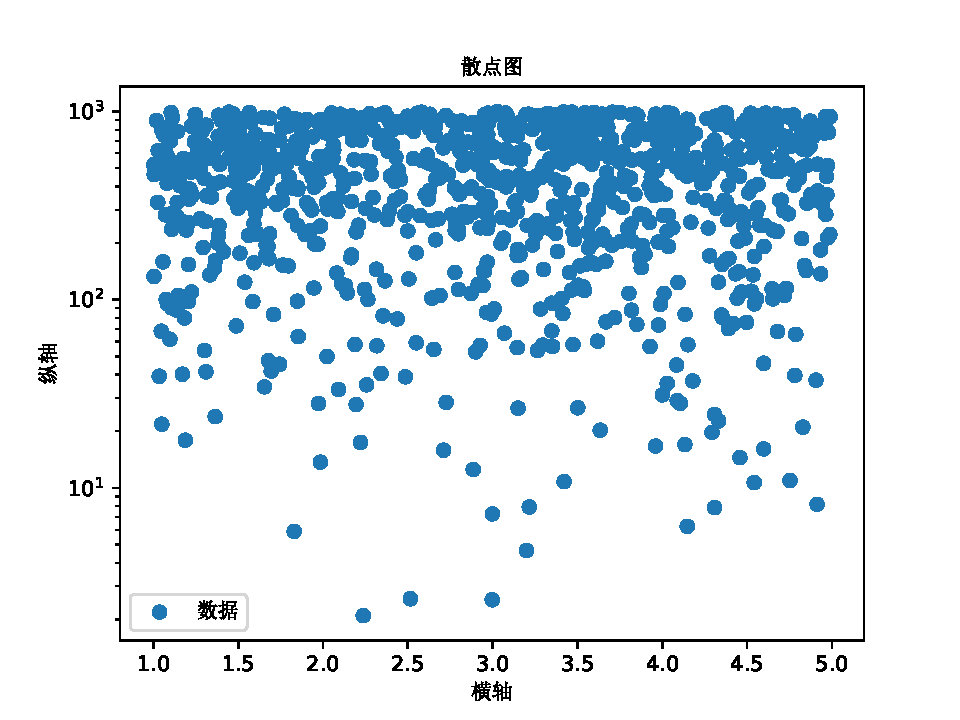
\includegraphics[width=0.45\linewidth]{figures/data/testA.pdf}}
	\quad %默认情况下两个子图之间空的较少,使用这个命令加大宽度
	\subfigure[level=9]{
		\label{level.sub.2}
		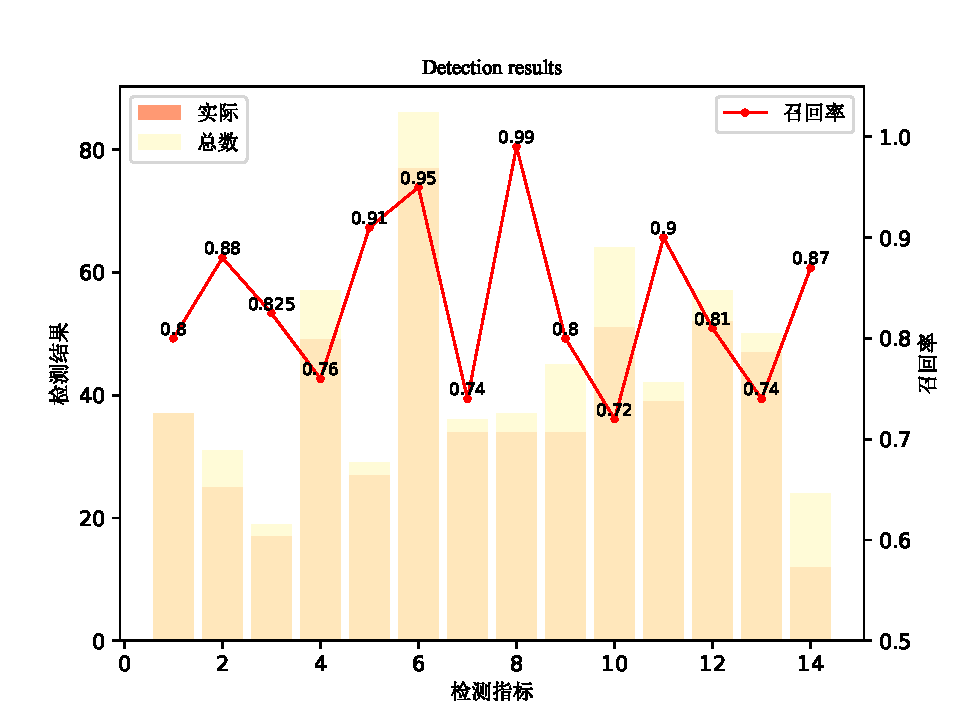
\includegraphics[width=0.45\linewidth]{figures/data/testB.pdf}}
	  %这里是空了一行,能够实现强制将四张图分成两行两列显示,而不是放不下图了再换行,使用\\也行。
	\caption{子图}
	\label{level}
\end{figure}

\section{公式}

行内公式,$p = q * \frac{q}{p}$,$\begin{bmatrix} a & b & c \end{bmatrix}$。

单行公式。

\begin{equation}
    e = \lim_{n\to \infty} \left(1 + \frac{1}{n}\right)^n
\end{equation}

多行公式~\ref{eq:foo}。

\begin{equation}
    \begin{aligned}
        1+ 1*2 - (2-1) & = 1+ 2 - 1 \\
                       & = 3-1      \\
                       & = 2
    \end{aligned}
    \label{eq:foo}
\end{equation}

多行公式,每行带序号
\begin{align}
  a & = b + c + d + e \\
    & = f + g
\end{align}


多行公式(无序号)。

\begin{equation*}
    \begin{aligned}
        1+ 1*2 - (2-1) & = 1+ 2 - 1 \\
                       & = 3-1      \\
                       & = 2
    \end{aligned}
\end{equation*}



\section{算法}

算法环境可以使用 \textbf{algorithms} 或者  \textbf{algorithm2e} 宏包。

\renewcommand{\algorithmicrequire}{\textbf{输入:}\unskip}
\renewcommand{\algorithmicensure}{\textbf{输出:}\unskip}



\section{本章小结}

